\documentclass[12pt, letterpaper]{../assignment}
\usepackage{graphicx}
\usepackage{courier}
\usepackage{minted}
\usepackage{amsmath}
\usepackage{polynom}
\usepackage{commath}
\usepackage{amssymb}
\usepackage{amsfonts} 
\usepackage{color}
\usepackage{cancel}
\usepackage{enumitem}
\usepackage{graphicx}
\usepackage{multirow}
\usepackage{float}
\usepackage{bm}
\usepackage{tikz}
\usetikzlibrary{shapes,arrows}
\usepackage{booktabs}
\usetikzlibrary{patterns}

% Define Theme Colors
\definecolor{light-gray}{rgb}{0.2,0.2,0.2}
\definecolor{header-blue}{rgb}{0,0,0.7}
% \definecolor{header-blue}{rgb}{0.5137,0.8353,0.9176}
\definecolor{header-blue}{rgb}{0,0.8,0.95}
\definecolor{dark-gray}{rgb}{0.1,0.1,0.1}
\pagecolor{dark-gray}
\color{white}

\usemintedstyle{monokai}
\oddsidemargin = 0pt
\exercisesheet{Module 9}{Assignment}
\student{Austin Barrilleaux}
\university{\color{header-blue}Johns Hopkins University}
\school{\color{header-blue}Whiting School of Engineering}
\courselabel{EN 535.612}
\semester{Fall 2024}
\usepackage[backend=bibtex,style=numeric,sorting=none]{biblatex}
\bibliography{reference}

\definecolor{light-gray}{rgb}{0.2,0.2,0.2}
\setminted{bgcolor=light-gray,frame=lines,rulecolor=white}
\setlength{\parindent}{0pt}

\makeatletter
\patchcmd{\minted@colorbg}{\noindent}{\medskip\noindent}{}{}
\apptocmd{\endminted@colorbg}{\par\medskip}{}{}
\makeatother

\begin{document}

\subsection*{Problem 1}
\subsubsection*{Derive the equations of motion for a rotating spring-pendulum shown below. The spring-
pendulum is attached at point $\bm{P}$.}

\begin{center}


    \tikzset{every picture/.style={line width=0.75pt}} %set default line width to 0.75pt        

    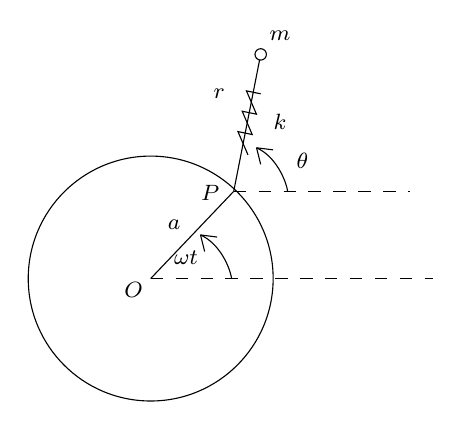
\begin{tikzpicture}[x=0.75pt,y=0.75pt,yscale=-1,xscale=1]
    %uncomment if require: \path (0,235); %set diagram left start at 0, and has height of 235
    
    %Shape: Circle [id:dp6807453817434252] 
    \draw   (56,146) .. controls (56,113.42) and (82.42,87) .. (115,87) .. controls (147.58,87) and (174,113.42) .. (174,146) .. controls (174,178.58) and (147.58,205) .. (115,205) .. controls (82.42,205) and (56,178.58) .. (56,146) -- cycle ;
    %Straight Lines [id:da7178841607482844] 
    \draw    (115,146) -- (155,104) ;
    %Straight Lines [id:da7998909593526187] 
    \draw  [dash pattern={on 4.5pt off 4.5pt}]  (115,146) -- (251,146) ;
    %Straight Lines [id:da8552075339271217] 
    \draw  [dash pattern={on 4.5pt off 4.5pt}]  (155,104) -- (240,104) ;
    %Straight Lines [id:da22269121285919313] 
    \draw    (155,104) -- (168,38) ;
    %Shape: Circle [id:dp3283193312313004] 
    \draw  [color={rgb, 255:red, 0; green, 0; blue, 0 }  ,draw opacity=1 ][fill={rgb, 255:red, 255; green, 255; blue, 255 }  ,fill opacity=1 ] (165.25,38) .. controls (165.25,36.48) and (166.48,35.25) .. (168,35.25) .. controls (169.52,35.25) and (170.75,36.48) .. (170.75,38) .. controls (170.75,39.52) and (169.52,40.75) .. (168,40.75) .. controls (166.48,40.75) and (165.25,39.52) .. (165.25,38) -- cycle ;
    %Shape: Sawtooth Wave Form [id:dp5568643638917725] 
    \draw   (161.87,86.43) -- (157.04,75.19) -- (163.91,76.62) -- (159.09,65.38) -- (165.96,66.81) -- (161.13,55.57) -- (168,57) ;
    %Curve Lines [id:da7874593699623249] 
    \draw    (166,83) .. controls (175,87) and (180,98) .. (181,104) ;
    %Straight Lines [id:da929282641989394] 
    \draw    (166,83) -- (168,91) ;
    %Straight Lines [id:da0375426544010975] 
    \draw    (166,83) -- (174,84) ;
    %Curve Lines [id:da41148044951051044] 
    \draw    (139,125) .. controls (148,129) and (153,140) .. (154,146) ;
    %Straight Lines [id:da7112124837478031] 
    \draw    (139,125) -- (141,133) ;
    %Straight Lines [id:da6585497222005503] 
    \draw    (139,125) -- (147,126) ;
    
    % Text Node
    \draw (125,131.4) node [anchor=north west][inner sep=0.75pt]  [font=\footnotesize]  {$\omega t$};
    % Text Node
    \draw (184,84.4) node [anchor=north west][inner sep=0.75pt]  [font=\footnotesize]  {$\theta $};
    % Text Node
    \draw (171,25.4) node [anchor=north west][inner sep=0.75pt]  [font=\footnotesize]  {$m$};
    % Text Node
    \draw (144,53.4) node [anchor=north west][inner sep=0.75pt]  [font=\footnotesize]  {$r$};
    % Text Node
    \draw (173,65.4) node [anchor=north west][inner sep=0.75pt]  [font=\footnotesize]  {$k$};
    % Text Node
    \draw (101,146.4) node [anchor=north west][inner sep=0.75pt]  [font=\footnotesize]  {$O$};
    % Text Node
    \draw (122,116.4) node [anchor=north west][inner sep=0.75pt]  [font=\footnotesize]  {$a$};
    % Text Node
    \draw (138,100) node [anchor=north west][inner sep=0.75pt]  [font=\footnotesize]  {$P$};
    
    
    \end{tikzpicture}
    
\end{center}

For this problem, the kinetic energy of the system, $T$, is defined as:

$$ T = \frac{1}{2} m v^2 $$

Therefore:

$$ T = \frac{1}{2} m \left(\dot{x}^2 + \dot{y}^2\right)  $$

By inspection of the sketch:

\begin{equation*}
    \begin{aligned}
    x &= a \cos(\omega t) + r\cos(\theta)\\
    y &= a \sin(\omega t) + r\sin(\theta)
    \end{aligned}
\end{equation*}

Taking the time derivative of both:

\begin{equation*}
    \begin{aligned}
    \dot{x} &= \dot{r}\cos\left(\theta\right)-r\,\dot{\theta}\sin\left(\theta\right)-a\,\omega \,\sin\left(\omega \,t\right) \\
    \dot{y} &= \dot{r}\sin\left(\theta\right)+r\,\dot{\theta}\cos\left(\theta\right)+a\,\omega \,\cos\left(\omega \,t\right)
    \end{aligned}
\end{equation*}

This gives:

$$ T = \frac{1}{2}\,m\,\left({\dot{r}}^2+{r}^2\,{\dot{\theta}}^2+a^2\,\omega ^2+2\,a\,\omega \,\sin\left(\theta -\omega \,t\right)\,\dot{r}+2\,a\,\omega \,r\,\cos\left(\theta -\omega \,t\right)\,\dot{\theta} \right)  $$

The potential energy of the system, $V$ is defined by:

$$ V = \frac{1}{2}k\left( r - r_0 \right)^2 $$


Given that the Lagrange is $ L = T - V $:

$$ L = \frac{1}{2}\,m\,\left({\dot{r}}^2+{r}^2\,{\dot{\theta}}^2+a^2\,\omega ^2+2\,a\,\omega \,\sin\left(\theta -\omega \,t\right)\,\dot{r}+2\,a\,\omega \,r\,\cos\left(\theta -\omega \,t\right)\,\dot{\theta} \right)
- \frac{1}{2}k\left( r - r_0 \right)^2  $$

We will solve for the equations of motion along the two generalized coordinates, $\theta$ and $r$.
Starting with $r$, we will solve:

$$ \frac{d}{d t} \frac{\partial L}{\partial \dot{r}} - \frac{\partial L}{\partial r} = 0 $$

The component parts of this equation are:

$$ \frac{\partial L}{\partial r} = 
m\,\left(r\,{\dot{\theta} }^2+a\,\omega \,\cos\left(\theta -\omega \,t\right)\,\dot{\theta} \right) -\,k\,\left(\,r-\,r_{0}\right) $$

$$ \frac{\partial L}{\partial \dot{r}}  =
m\,\left(\dot{r}+a\,\omega \,\sin\left(\theta -\omega \,t\right)\right) $$

$$ \frac{d}{d t} \frac{\partial L}{\partial \dot{r}} =
m\,\left(\ddot{r}-a\,\omega \,\cos\left(\theta -\omega \,t\right)\,\left(\omega -\dot{\theta} \right)\right) $$

This results in the equation of motion:

$$ \ddot{r}-r\,{\dot{\theta} }^2-a\,\omega ^2\,\cos\left(\theta -\omega \,t\right) + \frac{k}{m}\,(r-r_{0}) = 0 $$

Solving along $\theta$

$$ \frac{d}{d t} \frac{\partial L}{\partial \dot{\theta}} - \frac{\partial L}{\partial \theta} = 0 $$

The component parts of this equation are:

$$ \frac{\partial L}{\partial \theta} = 
m\,\left(a\,\omega \,\cos\left(\omega \,t-\theta \right)\,\dot{r}+a\,\omega \,\sin\left(\omega \,t-\theta \right)\,r\,\dot{\theta} \right) $$

$$ \frac{\partial L}{\partial \dot{\theta}}  =
,m\,\left({r}^2\,\dot{\theta} +a\,\omega \,\cos\left(\theta -\omega \,t\right)\,r\right) $$

$$ \frac{d}{d t} \frac{\partial L}{\partial \dot{\theta}} =
m\,\left({r}^2\,\ddot{\theta} +2\,r\,\dot{\theta} \,\dot{r}+a\,\omega \,\cos\left(\theta -\omega \,t\right)\,\dot{r}+a\,\omega \,r\,\sin\left(\theta -\omega \,t\right)\,\left(\omega -\dot{\theta} \right)\right) $$

This results in the equation of motion:

$$ r\,\ddot{\theta} +2\,\dot{\theta} \,\dot{r}+a\,\omega ^2\,\sin\left(\theta -\omega \,t\right) = 0  $$

The equations of motion for the system are:

\begin{answer}
\begin{equation*}
\begin{aligned}
\ddot{r}-r\,{\dot{\theta} }^2-a\,\omega ^2\,\cos\left(\theta -\omega \,t\right) + \frac{k}{m}\,(r-r_{0}) &= 0 \\
r\,\ddot{\theta} +2\,\dot{\theta} \,\dot{r}+a\,\omega ^2\,\sin\left(\theta -\omega \,t\right) &= 0 
\end{aligned}
\end{equation*}
\end{answer}

The following MATLAB script was used to solve this problem:

% \color{white}
\hspace*{6em}\inputminted[frame=leftline,fontsize=\footnotesize]{matlab}
{./matlab/Problem_1.m}
% \color{black} 

\subsection*{Problem 2}
\subsubsection*{Derive the equations of motion for the base-excited structure subject to an axial load $\bm{P(t)}$.}

\begin{center}
    \tikzset{every picture/.style={line width=0.75pt}} %set default line width to 0.75pt        
    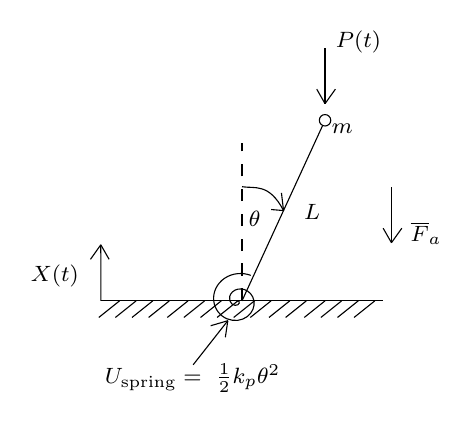
\begin{tikzpicture}[x=0.75pt,y=0.75pt,yscale=-1,xscale=1]
    %uncomment if require: \path (0,235); %set diagram left start at 0, and has height of 235
    %Straight Lines [id:da7988239387661931] 
    \draw    (85,161) -- (221,161) ;
    %Straight Lines [id:da433967165778121] 
    \draw    (84,169) -- (94,161) ;
    %Straight Lines [id:da3638550034994057] 
    \draw    (92,169) -- (102,161) ;
    %Straight Lines [id:da16117109148667996] 
    \draw    (100,169) -- (110,161) ;
    %Straight Lines [id:da4375189563254478] 
    \draw    (108,169) -- (118,161) ;
    %Straight Lines [id:da4196959967714724] 
    \draw    (117,169) -- (127,161) ;
    %Straight Lines [id:da604525149658292] 
    \draw    (125,169) -- (135,161) ;
    %Straight Lines [id:da7218062027735146] 
    \draw    (133,169) -- (143,161) ;
    %Straight Lines [id:da4011814914295413] 
    \draw    (141,169) -- (151,161) ;
    %Straight Lines [id:da4361083143725917] 
    \draw    (149,169) -- (159,161) ;
    %Straight Lines [id:da3771400943430454] 
    \draw    (157,169) -- (167,161) ;
    %Straight Lines [id:da4811503235326229] 
    \draw    (166,169) -- (176,161) ;
    %Straight Lines [id:da2562781992520886] 
    \draw    (174,169) -- (184,161) ;
    %Straight Lines [id:da6870325307074283] 
    \draw    (183,169) -- (193,161) ;
    %Straight Lines [id:da7783982945825645] 
    \draw    (191,169) -- (201,161) ;
    %Straight Lines [id:da20511703014012728] 
    \draw    (199,169) -- (209,161) ;
    %Straight Lines [id:da6029246345254777] 
    \draw    (207,169) -- (217,161) ;
    %Straight Lines [id:da2989222865393577] 
    \draw  [dash pattern={on 4.5pt off 4.5pt}]  (153,161) -- (153,85) ;
    %Straight Lines [id:da6331140346824675] 
    \draw    (153,161) -- (193,74) ;
    %Shape: Circle [id:dp2247586059899751] 
    \draw  [color={rgb, 255:red, 0; green, 0; blue, 0 }  ,draw opacity=1 ][fill={rgb, 255:red, 255; green, 255; blue, 255 }  ,fill opacity=1 ] (190.25,74) .. controls (190.25,72.48) and (191.48,71.25) .. (193,71.25) .. controls (194.52,71.25) and (195.75,72.48) .. (195.75,74) .. controls (195.75,75.52) and (194.52,76.75) .. (193,76.75) .. controls (191.48,76.75) and (190.25,75.52) .. (190.25,74) -- cycle ;
    %Curve Lines [id:da555130849372792] 
    \draw    (153,106) .. controls (159,107) and (166,104) .. (173,117.5) ;
    %Straight Lines [id:da35567044308417683] 
    \draw    (172,109) -- (173,117.5) ;
    %Straight Lines [id:da03561483139923505] 
    \draw    (167,117) -- (173,117.5) ;
    %Straight Lines [id:da813880146614568] 
    \draw    (193,66) -- (193,39) ;
    %Straight Lines [id:da949816246697498] 
    \draw    (189,59) -- (193,66) ;
    %Straight Lines [id:da5009384915479953] 
    \draw    (198,59) -- (193,66) ;
    %Shape: Spiral [id:dp1781996928710754] 
    \draw   (151,161) .. controls (151.24,161) and (151.42,161.1) .. (151.56,161.31) .. controls (151.7,161.53) and (151.73,161.79) .. (151.65,162.08) .. controls (151.55,162.41) and (151.33,162.67) .. (151,162.88) .. controls (150.63,163.11) and (150.19,163.2) .. (149.71,163.17) .. controls (149.16,163.12) and (148.66,162.92) .. (148.2,162.56) .. controls (147.69,162.16) and (147.33,161.64) .. (147.13,161) .. controls (146.9,160.3) and (146.88,159.57) .. (147.08,158.81) .. controls (147.31,157.99) and (147.76,157.28) .. (148.42,156.67) .. controls (149.13,156.01) and (150,155.58) .. (151,155.38) .. controls (152.07,155.15) and (153.15,155.22) .. (154.23,155.59) .. controls (155.37,155.97) and (156.35,156.63) .. (157.15,157.56) .. controls (158.01,158.55) and (158.53,159.69) .. (158.75,161) .. controls (158.98,162.38) and (158.81,163.73) .. (158.27,165.06) .. controls (157.7,166.46) and (156.78,167.63) .. (155.52,168.58) .. controls (154.2,169.57) and (152.69,170.17) .. (151,170.38) .. controls (149.23,170.59) and (147.51,170.35) .. (145.83,169.66) .. controls (144.09,168.94) and (142.64,167.82) .. (141.49,166.31) .. controls (140.29,164.74) and (139.59,162.97) .. (139.38,161) .. controls (139.15,158.95) and (139.48,156.97) .. (140.37,155.06) .. controls (141.3,153.08) and (142.68,151.45) .. (144.54,150.17) .. controls (146.46,148.85) and (148.61,148.08) .. (151,147.88) .. controls (153.14,147.69) and (155.21,147.97) .. (157.22,148.72) ;
    %Straight Lines [id:da2299544324594225] 
    \draw    (225,133) -- (225,106) ;
    %Straight Lines [id:da08869481177778638] 
    \draw    (221,126) -- (225,133) ;
    %Straight Lines [id:da26327615187069675] 
    \draw    (230,126) -- (225,133) ;
    %Straight Lines [id:da22452872090838816] 
    \draw    (146.16,170.57) -- (129.47,191.8) ;
    %Straight Lines [id:da8751075985411929] 
    \draw    (144.97,178.55) -- (146.16,170.57) ;
    %Straight Lines [id:da6619340703061136] 
    \draw    (137.9,172.99) -- (146.16,170.57) ;
    %Straight Lines [id:da8009572560395279] 
    \draw    (84.96,134) -- (85,161) ;
    %Straight Lines [id:da1426979973961593] 
    \draw    (88.97,140.99) -- (84.96,134) ;
    %Straight Lines [id:da7163454736261037] 
    \draw    (79.97,141.01) -- (84.96,134) ;
    % Text Node
    \draw (195,74.65) node [anchor=north west][inner sep=0.75pt]  [font=\footnotesize]  {$m$};
    % Text Node
    \draw (155,116.4) node [anchor=north west][inner sep=0.75pt]  [font=\footnotesize]  {$\theta $};
    % Text Node
    \draw (197,29.65) node [anchor=north west][inner sep=0.75pt]  [font=\footnotesize]  {$P( t)$};
    % Text Node
    \draw (233,121.65) node [anchor=north west][inner sep=0.75pt]  [font=\footnotesize]  {$\overline{F}_{a}$};
    % Text Node
    \draw (85.67,190.0) node [anchor=north west][inner sep=0.75pt]  [font=\footnotesize]  {$U_{\text{spring}} =\ \frac{1}{2} k_{p} \theta ^{2}$};
    % Text Node
    \draw (181.67,113.07) node [anchor=north west][inner sep=0.75pt]  [font=\footnotesize]  {$L$};
    % Text Node
    \draw (50,142.4) node [anchor=north west][inner sep=0.75pt]  [font=\footnotesize]  {$X(t)$};
    \end{tikzpicture}
\end{center}


For this problem, the kinetic energy of the system, $T$, is defined as:

$$ T = \frac{1}{2} m v^2 $$

Therefore:

$$ T = \frac{1}{2} m \left(\dot{x}^2 + \dot{y}^2\right)  $$

By inspection of the sketch:

\begin{equation*}
    \begin{aligned}
    x &= L\sin(\theta)\\
    y &= L\cos(\theta)
    \end{aligned}
\end{equation*}

Taking the time derivative of both:

\begin{equation*}
    \begin{aligned}
    \dot{x} &= L\,\cos\left(\theta \right)\,\dot{\theta}  \\
    \dot{y} &= -L\,\sin\left(\theta \right)\,\dot{\theta} 
    \end{aligned}
\end{equation*}

This gives:

$$ T = \frac{1}{2}m\,L^2\,{\dot{\theta}}^2  $$

The potential energy of the system, $V$ is defined by:

$$ V = \frac{1}{2} k_p \theta^2 + m a y $$


Given that the Lagrange is $ L = T - V $:

$$ L = \frac{1}{2}m\,L^2\,{\dot{\theta}}^2 - \left( \frac{1}{2} k_p \theta^2 + m a y \right)$$
% - \frac{1}{2}k\left( r - r_0 \right)^2  $$

We will solve for the equation of motion along the generalized coordinate, $\theta$:

$$ \frac{d}{d t} \frac{\partial L}{\partial \dot{\theta}} - \frac{\partial L}{\partial \theta} = Q_\theta $$

The component parts of this equation are:

$$ \frac{\partial L}{\partial \theta} = 
L\,m\,a\,\sin\left(\theta \right)-k_{p}\,\theta  $$

$$ \frac{\partial L}{\partial \dot{\theta}}  =
L^2\,m\,\dot{\theta}  $$

$$ \frac{d}{d t} \frac{\partial L}{\partial \dot{\theta}} =
L^2\,m\,\ddot{\theta}  $$

\begin{equation*}
\begin{aligned}
Q_\theta &= \sum_{k=1}^{N=3} F_k \frac{\partial x_k }{\partial \theta}\\
&=\left[\begin{array}{r} 0\\ -P\left(t\right) \end{array}\right] \cdot \left[\begin{array}{r} L\,\cos\left(\theta \right)\\ -L\,\sin\left(\theta \right) \end{array}\right]\\
&= L\sin(\theta(t)) P(t)
\end{aligned}
\end{equation*}

This results in the system equation of motion:

$$ m\,L^2\,\ddot{\theta} -m\,a\,\sin\left(\theta \right)\,L+k_{p}\,\theta  = L\ P(t)\ \sin(\theta)   $$

Or:

$$ m\,L\,\ddot{\theta} -m\,a\,\sin\left(\theta \right)+k_{p}\,\theta  = P(t)\ \sin(\theta)   $$


% \begin{answer}
% \begin{equation*}
% \begin{aligned}
% \ddot{r}-r\,{\dot{\theta} }^2-a\,\omega ^2\,\cos\left(\theta -\omega \,t\right) + \frac{k}{m}\,(r-r_{0}) &= 0 \\
% r\,\ddot{\theta} +2\,\dot{\theta} \,\dot{r}+a\,\omega ^2\,\sin\left(\theta -\omega \,t\right) &= 0 
% \end{aligned}
% \end{equation*}
% \end{answer}

The following MATLAB script was used to solve this problem:

% \color{white}
\hspace*{6em}\inputminted[frame=leftline,fontsize=\footnotesize]{matlab}
{./matlab/Problem_1.m}
% \color{black} 


\subsection*{Problem 3}
\subsubsection*{The double pendulum. Find the equations governing a rigid bar attached to a string as shown
in the figure.}

\begin{center}
\tikzset{every picture/.style={line width=0.75pt}} %set default line width to 0.75pt        
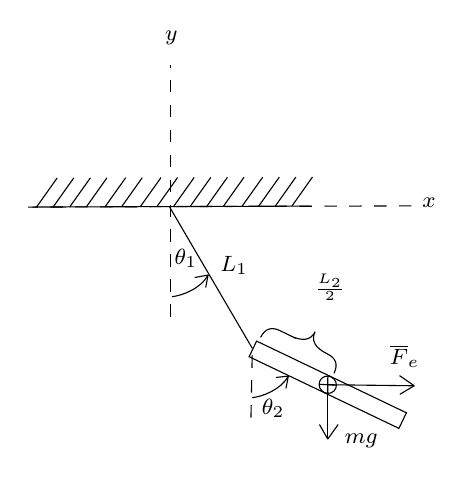
\begin{tikzpicture}[x=0.75pt,y=0.75pt,yscale=-1,xscale=1]
%uncomment if require: \path (0,235); %set diagram left start at 0, and has height of 235
%Straight Lines [id:da5098103873800055] 
\draw    (217.02,98.76) -- (81.02,99.24) ;
%Straight Lines [id:da9938488817744722] 
\draw    (217.97,84.76) -- (208.02,98.8) ;
%Straight Lines [id:da6448556991299332] 
\draw    (209.97,84.79) -- (200.02,98.82) ;
%Straight Lines [id:da5578613159239434] 
\draw    (201.98,84.82) -- (192.02,98.85) ;
%Straight Lines [id:da5578580802015525] 
\draw    (193.98,84.84) -- (184.02,98.88) ;
%Straight Lines [id:da6878242170016136] 
\draw    (184.98,84.88) -- (175.02,98.91) ;
%Straight Lines [id:da576088509348444] 
\draw    (176.98,84.9) -- (167.02,98.94) ;
%Straight Lines [id:da36538893944236794] 
\draw    (168.98,84.93) -- (159.02,98.97) ;
%Straight Lines [id:da519347545292852] 
\draw    (160.98,84.96) -- (151.02,98.99) ;
%Straight Lines [id:da9815318743859791] 
\draw    (152.98,84.99) -- (143.02,99.02) ;
%Straight Lines [id:da4749097207634776] 
\draw    (144.98,85.02) -- (135.02,99.05) ;
%Straight Lines [id:da18642908080287368] 
\draw    (135.98,85.05) -- (126.02,99.08) ;
%Straight Lines [id:da19351022301219567] 
\draw    (127.98,85.08) -- (118.02,99.11) ;
%Straight Lines [id:da8783946704150984] 
\draw    (118.98,85.11) -- (109.02,99.14) ;
%Straight Lines [id:da20643960149931906] 
\draw    (110.98,85.13) -- (101.02,99.17) ;
%Straight Lines [id:da9234111571632202] 
\draw    (102.98,85.16) -- (93.02,99.2) ;
%Straight Lines [id:da3696883349295832] 
\draw    (94.98,85.19) -- (85.02,99.23) ;
%Straight Lines [id:da0328362287292987] 
\draw  [dash pattern={on 4.5pt off 4.5pt}]  (149.67,152) -- (149.67,30.67) ;
%Straight Lines [id:da1481348133865612] 
\draw  [dash pattern={on 4.5pt off 4.5pt}]  (265.67,98.67) -- (83.02,99.23) ;
%Straight Lines [id:da009693355497953249] 
\draw    (189,167.33) -- (149.02,99) ;
%Curve Lines [id:da8370150143762951] 
\draw    (167.67,132) .. controls (164.1,138.59) and (155.12,141.9) .. (150.3,142.41) ;
%Straight Lines [id:da6097109608235824] 
\draw    (167.67,132) -- (161.21,133.18) ;
%Straight Lines [id:da11669008040890394] 
\draw    (167.67,132) -- (166.53,137.96) ;
%Flowchart: Process [id:dp7868041789682514] 
\draw   (191.05,163.81) -- (263.21,198.34) -- (259.62,205.86) -- (187.45,171.33) -- cycle ;
%Flowchart: Summing Junction [id:dp8667190641446441] 
\draw   (222.37,187.64) .. controls (220.75,185.94) and (220.77,183.3) .. (222.41,181.75) .. controls (224.05,180.2) and (226.68,180.32) .. (228.3,182.03) .. controls (229.91,183.73) and (229.89,186.37) .. (228.26,187.92) .. controls (226.62,189.47) and (223.98,189.35) .. (222.37,187.64) -- cycle ; \draw   (221.17,184.64) -- (229.5,185.03) ; \draw   (225.36,180.67) -- (225.3,189) ;
%Straight Lines [id:da8749134080912189] 
\draw    (225.33,211) -- (225.33,184) ;
%Straight Lines [id:da35716800657131986] 
\draw    (221.33,204) -- (225.33,211) ;
%Straight Lines [id:da38589321373121077] 
\draw    (230.33,204) -- (225.33,211) ;
%Straight Lines [id:da38000904259491763] 
\draw  [dash pattern={on 4.5pt off 4.5pt}]  (188.33,200.67) -- (189,167.33) ;
%Curve Lines [id:da7142830592624412] 
\draw    (206.33,180.67) .. controls (202.76,187.25) and (193.79,190.56) .. (188.96,191.07) ;
%Straight Lines [id:da5422226822777882] 
\draw    (206.33,180.67) -- (205.2,186.62) ;
%Straight Lines [id:da682557586296844] 
\draw    (200.33,181.33) -- (206.33,180.67) ;
%Straight Lines [id:da9604866227989712] 
\draw    (267,185.33) -- (225.33,184.83) ;
%Straight Lines [id:da4673576100259076] 
\draw    (260.06,189.44) -- (267,185.33) ;
%Straight Lines [id:da5086437465815203] 
\draw    (259.92,180.44) -- (267,185.33) ;
%Shape: Brace [id:dp42576135699371553] 
\draw   (228.33,179.33) .. controls (230.39,175.14) and (229.32,172.02) .. (225.13,169.97) -- (225.13,169.97) .. controls (219.14,167.03) and (217.18,163.47) .. (219.24,159.28) .. controls (217.18,163.47) and (213.16,164.09) .. (207.18,161.16)(209.87,162.48) -- (202.37,158.8) .. controls (198.18,156.75) and (195.05,157.81) .. (193,162) ;

% Text Node
\draw (150.33,118.4) node [anchor=north west][inner sep=0.75pt]  [font=\footnotesize]  {$\theta _{1}$};
% Text Node
\draw (232.33,207.4) node [anchor=north west][inner sep=0.75pt]  [font=\footnotesize]  {$mg$};
% Text Node
\draw (192.33,190.4) node [anchor=north west][inner sep=0.75pt]  [font=\footnotesize]  {$\theta _{2}$};
% Text Node
\draw (254,164.32) node [anchor=north west][inner sep=0.75pt]  [font=\footnotesize]  {$\overline{F}_{e}$};
% Text Node
\draw (172.33,121.73) node [anchor=north west][inner sep=0.75pt]  [font=\footnotesize]  {$L_{1}$};
% Text Node
\draw (217.67,130.4) node [anchor=north west][inner sep=0.75pt]  [font=\scriptsize]  {$\frac{L_{2}}{2}$};
% Text Node
\draw (269.67,93.73) node [anchor=north west][inner sep=0.75pt]  [font=\footnotesize]  {$x$};
% Text Node
\draw (145.67,13.07) node [anchor=north west][inner sep=0.75pt]  [font=\footnotesize]  {$y$};


\end{tikzpicture}

\end{center}

\subsubsection*{a. This system starts with 9 degrees of freedom. What constraints exist that reduce this system to
only two degrees of freedom?}
\subsubsection*{b. Show that the Lagrangian is:
$$ \footnotesize \bm{L = \frac{1}{2}m\left[
    L_1^2 \dot{\theta}_1^2 +
    L_1 L_2 \dot{\theta}_1 \dot{\theta}_2 \cos(\theta_2-\theta_1) + 
    \frac{1}{3} {L}_2^2 \dot{\theta}_2^2
\right] - 
mg\left[ L_1 \left( 1 - \cos \ \theta_1  \right) + 
\frac{L_2}{2} \left( 1 - \cos\ \theta_2  \right)\right]} $$ }

For this problem, the kinetic energy of the system, $T$, is defined as:

$$ T = \frac{1}{2} m v^2 + \frac{1}{2} I \dot{\theta}_2^2 $$

Therefore:

$$ T = \frac{1}{2} m \left(\dot{x}^2 + \dot{y}^2\right) + \frac{1}{2}\left(\frac{1}{12}\right) L_2^2 \dot{\theta}_2^2 $$

By inspection of the sketch:

\begin{equation*}
\begin{aligned}
x &= L_1 \sin(\theta_1)+ \frac{L_2}{2} \sin(\theta_2)\\
y &= \left(L_1 + \frac{L_2}{2}\right) - L_1 \cos(\theta_1)- \frac{L_2}{2}\cos(\theta_2)
\end{aligned}
\end{equation*}

Note that these equations define $(x,y)_0$ at the location of the c.g. of the bar when $\theta_1 = \theta_2 = 0$.
\\\\

Taking the time derivative of both:

\begin{equation*}
    \begin{aligned}
    \dot{x} &= L_{1}\,\cos\left(\theta _{1}\right)\,\dot{\theta} _{1}+\frac{1}{2}\,L_{2}\,\cos\left(\theta _{2}\right)\,\dot{\theta} _{2} \\
    \dot{y} &= L_{1}\,\sin\left(\theta _{1}\right)\,\dot{\theta} _{1}+\frac{1}{2}\,L_{2}\,\sin\left(\theta _{2}\right)\,\dot{\theta} _{2}
    \end{aligned}
\end{equation*}

This gives:

$$ T = \frac{1}{2}\,m\,\left[{L_{1}}^2\,{\dot{\theta} _{1}}^2
+L_{1}\,L_{2}\,\dot{\theta} _{2}\,\dot{\theta} _{1}\cos\left(\theta _{2}-\theta _{1}\right)
+\frac{1}{3}\,{L_{2}}^2\,{\dot{\theta} _{2}}^2\right] $$

The potential energy of the system, $V$ is defined by:

$$ V = mgh $$

Therefore:

\begin{equation*}
    \begin{aligned}
    V &= m g \left(L_{1}+\frac{1}{2}\,L_{2}-L_{1}\,\cos\left(\theta _{1}\right)-\frac{1}{2}\,L_{2}\,\cos\left(\theta _{2}\right)\right) \\
    &= m g \left[L_{1}\,\left(1-\cos\left(\theta _{1}\right)\right)+\frac{1}{2} L_{2}\left(1-\,\cos\left(\theta _{2}\right)\right)\right]
    \end{aligned}
\end{equation*}


Given that the Lagrange is $ L = T - V $:

\begin{answer}
\begin{equation*}
\begin{aligned}
            L = \frac{1}{2}\,m\,&\left[{L_{1}}^2\,{\dot{\theta} _{1}}^2
+L_{1}\,L_{2}\,\dot{\theta} _{2}\,\dot{\theta} _{1}\cos\left(\theta _{2}-\theta _{1}\right)
+\frac{1}{3}\,{L_{2}}^2\,{\dot{\theta} _{2}}^2\right]\\
&- m g \left[L_{1}\,\left(1-\cos\left(\theta _{1}\right)\right)+\frac{1}{2} L_{2}\left(1-\,\cos\left(\theta _{2}\right)\right)\right]
\end{aligned}
\end{equation*}
\end{answer}

This matches the Lagrangian in the question prompt.

\subsubsection*{c. Use Lagrange's equations to derive the equations of motion (don't forget about the external
force!)}

Looking at the external forces:




% % \color{white}
% \hspace*{6em}\inputminted[frame=leftline,fontsize=\footnotesize]{matlab}
% {./matlab/Q6_8.m}
% % \color{black} 

% \begin{figure}[H]
%     \centering
%     \includegraphics[scale=0.7,frame]{images/Q5_13.png}
% \end{figure}




\end{document}

